%------------------------------------------------
\section{Méthodes de calculs existantes}
%------------------------------------------------

%-----------------------------------------------------------------
\subsection{Suivi de Bord}
%-----------------------------------------------------------------

La méthode du suivi du bord d'un disque discret est un processus étudié et connu. Elle est sensiblement la même suivant le cas souhaité : 4-connexes ou 8-connexes. Elle se décompose en deux étapes. Trouver un point sur le bord, puis chercher le point suivant de manière répétée jusqu'à retrouver le premier point et refermer le bord.

%-----------------------------------------------------------------
%\subsubsection{Trouver le sommet de départ}

Pour chercher un point de départ sur le bord du disque discret à partir de la seule connaissance de ses paramètres, nous avons choisi de récupérer le point d'ordonnée minimale et d'abscisse maximale à l'intérieur du disque. Nous prenons le point de $\mathbb{Z}^2$ avec les coordonnées entières du centre du disque. Puis, nous descendons le long de l'axe vertical d'une longueur entière égale au rayon pour trouver un point d'ordonnée miniamle. Ensuite, nous translatons suivant l'axe horizontal afin de récupérer le point d'abscisse maximal. On note \textbf{a} ce point de départ. Cette procédure prend un temps constant. 

\begin{figure}[H]
  \centering
  \includegraphics[width=0.3\linewidth,page=1]{fig/4-exi/suivi/exi-depart-0.pdf}
  \includegraphics[width=0.3\linewidth,page=1]{fig/4-exi/suivi/exi-depart-1.pdf}
  \caption{Recherche de $a$.}
\end{figure}
  

%-----------------------------------------------------------------
%\subsubsection{Trouver le sommet suivant}

La deuxième étape consiste à trouver le sommet suivant appartenant au bord. On répète cette étape jusqu'à retrouver le point a.

A partir d'un point quelconque du bord $p$ ($a$ au début), le point suivant est choisi suivant la position des 4 voisins (resp 8 voisins) de $p$ par rapport au disque et d'un sens arbitraire de rotation. En tournant dans le sens trigonométrique et en partant d'un voisin situé à l'extérieur du disque, le point suivant est le premier voisin situé à l'intérieur du disque. 

\begin{figure}[H]
  \centering
  \includegraphics[width=0.4\linewidth,page=1]{fig/4-exi/suivi/exi-suivi-0.pdf}
  \caption{Suivi de bord 4-connexes et 8-connexes}
\end{figure}
  
Cette étape prend un temps constant, limité par la taille constante du voisinage. Elle est répétée autant de fois qu'il y a de points sur le bord du disque. Rappelons que $R$ est le rayon du disque. Comme il y a $O(R)$ points sur le bord du disque, la complexité en temps du suivi est en $O(R)$. 

%-----------------------------------------------------------------
\subsection{Enveloppe Convexe : Algorithme de Har-Peled}
%-----------------------------------------------------------------

De nombreux algorithmes existent pour calculer l'enveloppe convexe d'un ensemble de points. L'algorithme de Graham l'implémente en $O(n \log n)$ pour un ensemble quelconque de $n$ points. Quand les $n$ points sont ordonnés, comme le sont les points du bord d'un disque discret, le parcours de Graham est en $O(n)$. Par conséquent, calculer l'enveloppe convexe des points d'un disque discret se calcule par suivi de bord et parcours de Graham en $O(R)$. Cependant un algorithme géométrique introduit par Har-Peled en 1998 calcule l'enveloppe convexe des points d'un disque discret de manière incrémentale et ``output-sensitive''.
%% reference pour Graham
%% reference pour Har-Peled

\begin{Definition}{Output sensitive}\\
\label{def:os}
      Un algorithme output sensitive possède un temps d’exécution qui dépend de la taille de sa sortie.
\end{Definition}

La méthode de Har-Peled dépend du nombre de sommets de l'enveloppe convexe. Elle construit successivement les arêtes du polygone à l'aide des convergents qui représente le pendant géométrique du calcul du pgcd de deux nombres entiers (voir l'annexe \ref{annexe-euc-geo}). La complexité en temps de cet algorithme pour un disque de rayon $R$ relève d'une part de la recherche du prochain sommet en $O(\log R)$ et également du nombre de sommets qui est $O(R^{2/3})$. Soit une complexité totale en temps de $O( R^{2/3} \log R)$.

%-----------------------------------------------------------------
\subsubsection{Calcul des convergents}

Cette méthode de calcul est géométrique. Soient l’origine $O=(0,0)$ et $P = (P_x, P_y)$ un point à coordonnées entières. Nous cherchons le premier point de $\mathbb{Z}^{2}$ appartenant au segment de droite [O,P]. Le coefficient trouvé correspond au pgcd de $P_x$ et $P_y$.\\

Soient $p_{-2} = (1,0)$ et $p_{-1} = (0,1)$ les deux premiers convergents. Pour trouver les convergents suivants, nous mettons en place une méthode récursive :

$$p_{k} = p_{k-2} + q_k p_{k-1}$$

où $q_k$ est le plus grand entier tel que $p_{k}$ et $p_{k-2}$ soient du même côté de la droite.\\

L'opération correspond à jeter un rayon de $p_{k-2}$ dans la direction de $p_{k-1}$ pour étudier l’intersection du vecteur et du segment de droite de direction $y_P / x_P$. La méthode s’arrête quand un convergent $p_{k}$ est exactement sur la droite.\\

\begin{figure}[H]
  \centering
  \includegraphics[width=0.4\linewidth]{fig/4-exi/har/exi-har-0.pdf}
  \includegraphics[width=0.4\linewidth]{fig/4-exi/har/exi-har-1.pdf}
  \caption{Calcul des convergents du point (3,8)}
\end{figure}


%% TRI: je ne vois pas l'intérêt ici: en annexe ?
%% \begin{table}[H]
%%   \centering
%%   \begin{tabular}{|p{0.04\linewidth}|p{0.04\linewidth}|p{0.04\linewidth}||p{0.04\linewidth}|p{0.04\linewidth}||p{0.2\linewidth}||p{0.35\linewidth}|}
%%     \hline 
%%     $k$ & $a$ & $b$ & $q_{k}$ & $r_k$ & (a,b) & $p_k$ \\
%%     \hline 
%%     -2 & - & - & - & - & -                    & $p_{-2} = (1,0)$\\
%%     -1 & - & - & - & - & $3 p_{-2} + 8p_{-1}$ & $p_{-1} = (0,1)$\\
%%      0 & 8 & 3 & 2 & 2 & $2 p_{-1} + 3p_{0}$  & $p_{0}  = p_{-2} + 2p_{-1} = (1,2)$\\ 
%%      1 & 3 & 2 & 1 & 1 & $p_{0}  + 2p_{1}$    & $p_{1}  = p_{-1} + p_{0} = (1,3)$\\
%%      2 & 2 & 1 & 2 & 0 & $p_{2}$              & $p_{2}  = p_{0} + 2p_{1} = (3,8)$\\
%%     \hline
%%   \end{tabular} 
%%   \caption{Résultat du $PGCD(3,8)$ par la méthode d'Euclide et géométrique}
%% \end{table}


%relié le tout à la fraction continue et revenir un peu à la méthode d'Euclide.

%-----------------------------------------------------------------
\subsubsection{Passage au disque}


La méthode de calcul de l'enveloppe convexe d'un disque se décompose en deux étapes. La première consiste à trouver un point de départ. Nous appliquons la même procédure que lors du suivi de bord pour récupérer le point de départ d'ordonnée minimale et d'abscisse maximale. Par définition ce point appartient à l'enveloppe convexe.\\

Ensuite, nous cherchons le sommet suivant jusqu'à retrouver le point de départ. Cette étape est réalisée en calculant les convergents les plus proches du bord du disque. Nous allons alternativement être à l'intérieur du disque lorsque $k$ est impair et à l'extérieur du disque lorsque $k$ est pair. Nous repartons d'un convergent s'il se situe exactement sur le bord du disque. Sinon, nous repartons du dernier convergent de degré impair lorsque que le lancer de rayon n'est pas effectif.\\
%% effectif: pas clair 
%% liens avec la figure ?

\begin{figure}[H]
  \centering
  \includegraphics[width=0.4\linewidth]{fig/4-exi/har/exi-har-10.pdf}
  \includegraphics[width=0.4\linewidth]{fig/4-exi/har/exi-har-11.pdf}
  \caption{Calcul de l'enveloppe convexe d'un disque}
\end{figure}

\subsubsection{Résultats}

Les résultats suivants ont été obtenus en calculant sur une moyenne de 100 disques de rayon $2^k$ possédant un centre à coordonnée rationnel compris dans $[0,1]\times[0,1]$. Afin de vérifier la convergence en $O(R^{2/3})$, nous avons également récupéré la moyenne par rayon de la division du nombre de sommets de l'enveloppe convexe sur le rayon à la puissance 2/3. La zone bleue de la figure correspond à l'intervale entre le minimum et le maximum obtenu.

On s'intéresse également à vérifié la complexité en temps de notre algorithme. On le compare notamment à la marche de Graham. 

\begin{figure}[H]
  \centering
  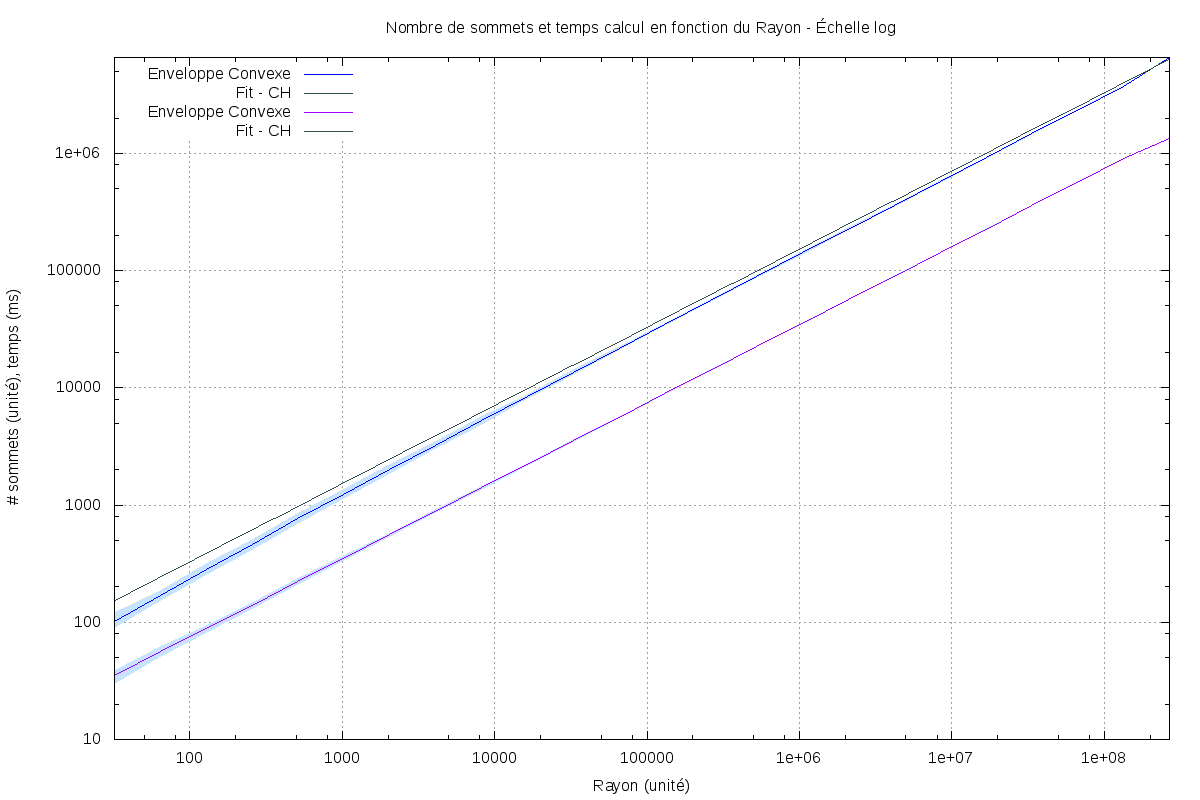
\includegraphics[width=\linewidth]{fig/4-exi/ch/exi-ch-sommet.png}
  \caption{Sommets et bord de l'enveloppe convexe}
\end{figure}

\begin{table}[H]
  \begin{tabular}{|p{0.09\linewidth}|p{0.13\linewidth}||p{0.2\linewidth}|p{0.13\linewidth}||p{0.2\linewidth}|p{0.13\linewidth}|}
    \hline
    \multicolumn{2}{|c||}{Rayon} & \multicolumn{4}{c|}{Enveloppe convexe} \\  \hline 
    $R=2^k$  &  & \multicolumn{2}{c||}{Nombre de Sommets} &  \multicolumn{2}{c|}{Nombre de points sur le bord} \\ \hline 
    k & R &   & $\# / R^{2/3}$  &   & $\# / R^{2/3}$ \\    
    \hline
    5 & 32         & 35,36     & 3,51 & 102,05   &  10,12\\
    6 & 64         & 55,78     & 3,49 & 170,16   &  10,64\\
    7 & 128        & 87,78     & 3,46 & 283,69   &  11,17\\
    8 & 256        & 139,71    & 3,47 & 465,06   &  11,53\\
    9 & 512        & 222,07    & 3,47 & 761,01   &  11,89\\
    10 & 1024      & 351,72    & 3,46 & 1,24E+03 &  12,21\\
    11 & 2048      & 558,18    & 3,46 & 2,01E+03 &  12,45\\
    12 & 4096      & 883,86    & 3,45 & 3,24E+03 &  12,68\\
    13 & 8192      & 1,40E+003 & 3,45 & 5,25E+03 &  12,92\\
    14 & 16384     & 2,23E+003 & 3,45 & 8,41E+03 &  13,03\\
    15 & 32768     & 3,54E+003 & 3,45 & 1,35E+04 &  13,19\\
    16 & 65536     & 5,62E+003 & 3,46 & 2,16E+04 &  13,28\\
    17 & 131072    & 8,91E+003 & 3,45 & 3,47E+04 &  13,45\\
    18 & 262144    & 1,41E+004 & 3,45 & 5,54E+04 &  13,53\\
    19 & 524288    & 2,25E+004 & 3,45 & 8,87E+04 &  13,64\\
    20 & 1048576   & 3,56E+004 & 3,45 & 1,42E+05 &  13,75\\
    21 & 2097152   & 5,66E+004 & 3,45 & 2,26E+05 &  13,81\\
    22 & 4194304   & 8,98E+004 & 3,45 & 3,61E+05 &  13,88\\
    23 & 8388608   & 1,43E+005 & 3,45 & 5,76E+05 &  13,94\\
    24 & 16777216  & 2,26E+005 & 3,45 & 9,19E+05 &  14,02\\
    25 & 33554432  & 3,59E+005 & 3,45 & 1,46E+06 &  14,07\\
    26 & 67108864  & 5,70E+005 & 3,45 & 2,33E+06 &  14,10\\
    27 & 134217728 & 8,98E+005 & 3,42 & 3,74E+06 &  14,27\\
    28 & 268435456 & 1,35E+06  & 3,24 & 6,62E+06 &  15,90\\
    \hline
  \end{tabular} 
  \caption{Sommet et bord de l'enveloppe convexe}
\end{table}

\begin{figure}[H]
  \centering
  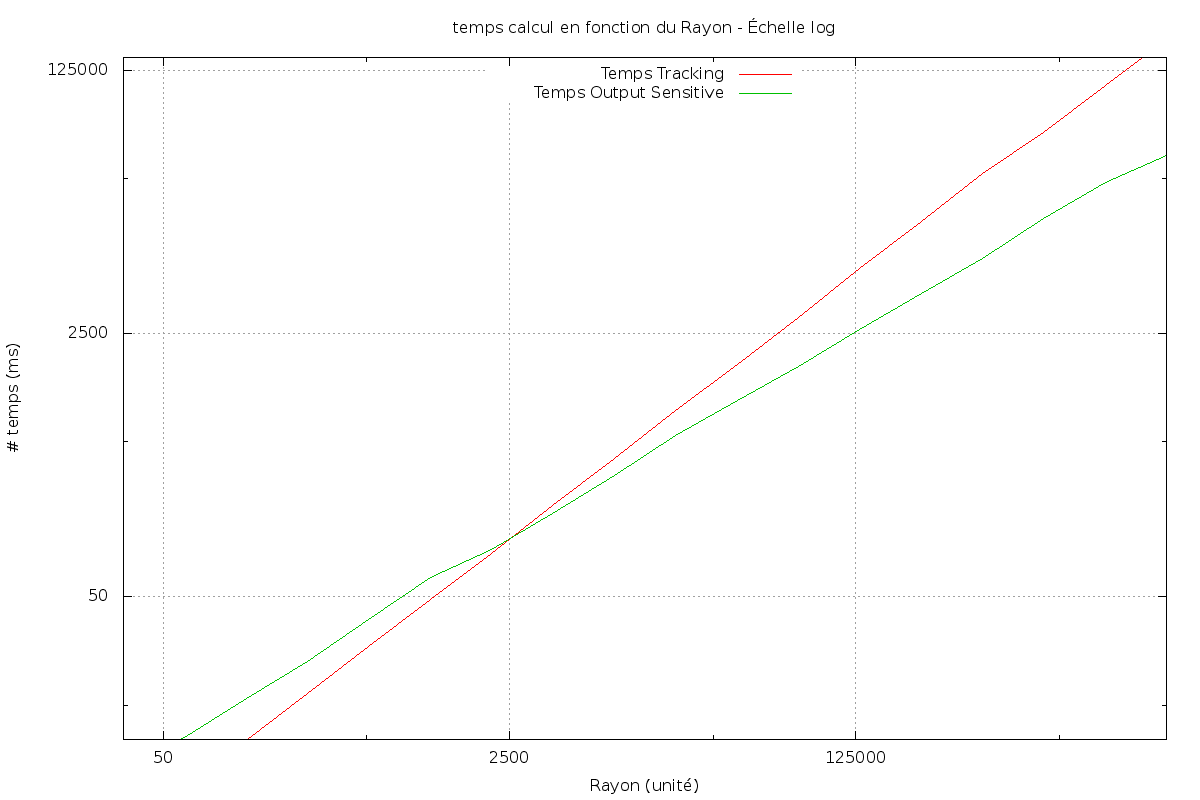
\includegraphics[width=\linewidth]{fig/4-exi/ch/exi-ch-temps.png}
  \caption{Temps de calcul de l'enveloppe convexe (échelle log / log)}
\end{figure}

%%TRI: non pertinent
%% \begin{table}[H]
%%   \begin{tabular}{|p{0.09\linewidth}|p{0.13\linewidth}||p{0.23\linewidth}|p{0.23\linewidth}|p{0.23\linewidth}|}
%%     \hline
%%     \multicolumn{2}{|c||}{Rayon} & \multicolumn{3}{c|}{Temps de calcul (ms) } \\  \hline 
%%     $R=2^k$  &  &  \multicolumn{3}{c|}{Enveloppe Convexe}  \\ \hline
%%     k & R & Marche de Grahaam & Har-Peled - Sommets & Har-Peled - Bord \\
%%     \hline
%%     5  & 32        & 0,64     & 1,05     & 1,98\\
%%     6  & 64        & 1,18     & 1,87     & 3,77\\
%%     7  & 128       & 2,33     & 3,3      & 7,08\\
%%     8  & 256       & 4,64     & 5,86     & 13,02\\
%%     9  & 512       & 9,25     & 10,29    & 23,99\\
%%     10 & 1024      & 32,5     & 17,9     & 43,34\\
%%     11 & 2048      & 37,03    & 31,13    & 78,05\\
%%     12 & 4096      & 74,55    & 53,75    & 139,12\\
%%     13 & 8192      & 149,03   & 92,57    & 247,36\\
%%     14 & 16384     & 297,79   & 159,44   & 433,88\\
%%     15 & 32768     & 596,22   & 272,74   & 760,20\\
%%     16 & 65536     & 1,19E+03 & 466,51   & 1,32E+03\\
%%     17 & 131072    & 2,37E+03 & 795,09   & 2,30E+03\\
%%     18 & 262144    & 4,73E+03 & 1,35E+03 & 3,99E+03\\
%%     19 & 524288    & 9,47E+03 & 2,29E+03 & 6,88E+03\\
%%     20 & 1048576   & 1,89E+04 & 3,88E+03 & 1,18E+04\\
%%     21 & 2097152   & 3,79E+04 & 6,58E+03 & 2,02E+04\\
%%     22 & 4194304   & 7,58E+04 & 1,11E+04 & 3,45E+04\\
%%     23 & 8388608   & 1,52E+05 & 1,86E+04 & 5,88E+04\\
%%     24 & 16777216  & 3,03E+05 & 3,13E+04 & 1,00E+05\\
%%     25 & 33554432  & 6.04E+05 & 5,26E+04 & 1,70E+05\\
%%     26 & 67108864  & 1.20E+06 & 8,80E+04 & 2,87E+05\\
%%     27 & 134217728 & 2.42E+06 & 1,46E+05 & 4,82E+05\\
%%     28 & 268435456 &          & 2,33E+05 & 8,85E+05\\
%%     \hline
%%   \end{tabular} 
%%   \caption{Temps de calcul de l'enveloppe convexe}
%% \end{table}
%%

Nos résultats obtenus sont conformes à ceux de la publication \cite{HarPeled98}. On remarque que la moyenne asymptotique de la division du nombre moyen de sommets de l'enveloppe convexe sur le rayon à la puissance 2/3 est 3,45. Des anomalies commencent à apparaître pour des rayons de la taille de $2^{27} = 134217728$. Il convient de chercher à comprendre d'où elles viennent afin de mieux cerner les possibles limitations de notre algorithme.\\

Le graphique représentant les temps est également intéressant. On observe avec l'échelle logarithmique que la complexité en temps est sous-linéaire pour la méthode de Har-Peled. La méthode devient d'ailleurs plus intéressante que la marche de Grahaam en terme de temps de calcul assez rapidement à partir d'un rayon $2^{10} = 1024$ unités. 
% alors que la méthode qui récupère également les points sur les sommets devient plus rapide qu'à partir de $2^{17} = 131072$.
%% TRI: non pertinent, enlevé la courbe de temps avec les points sur le bord



